\chapter{Desarrollo de la investigaci\'on}

Este cap\'itulo comprende la exposici\'on detallada del desarrollo de versi\'on final del \textit{software}  siguiendo una metodolog\'ia en espiral; se describe las diferentes iteraciones del ciclo y las fases de la elaboraci\'on del \textit{software} al que se denomin\'o HIVmlm (Human Immunology Virus linear model mixed effects).\\

\section{Desarrollo}

Siguiendo la metodolog\'ia de trabajo en espiral, se construy\'o  una lista de los m\'odulos a desarrollar en la aplicaci\'on acorde a los objetivos planteados en la investigaci\'on, y siguiendo los paradigmas para el desarrollo de paquetes en lenguaje R, presentados por \citet{test} y por el creador del paquete \emph{formatR} \citet{format}. Los m\'odulos desarrollados fueron:


\begin{enumerate}
\item Carga de datos
\item Exploraci\'on de los datos
\item Visualizaci\'on en el mapa
\item Ajuste del m\'odelo
\item Validaci\'on del m\'odelo
\item Generar reporte
\end{enumerate}
   
 Cada m\'odulo paso por las etapas del m\'odelo en espiral, en este caso, 4 etapas planificadas, estas etapas se realizaron dentro del tiempo establecido, con una revision semanal por parte de la tutora, dichas etapas se detallar\'an a continuaci\'on:

\section{Etapa 1}

Siguiendo cada una de las etapas de la metodologóa en espiral el desarrollo de \textit{software}, se comienza por el an\'alisis de riesgo y el dise\~no de prototipos. Para el desarrollo de la aplicaci\'on se seleccion\'o Lenguaje R. \\

Los m\'etodos para el dise\~no de las funciones primarias en R ser\'an los diagramas de flujo; y para su codificaci\'on se seguir\'an las normas de estilo para codificaci\'on en R, sugeridas por \citet{test} y por el creador del paquete \emph{formatR} \citet{format}, adem\'as se establecer\'an la dependencia con las funciones de c\'odigo base y las recomendadas para desarrollo en R.\\

Se desarroll\'o el m\'odulo de Carga de Datos  asociados a los  pacientes, primero se filtr\'o la informaci\'on para el caso de estudio, la cual  pertenece a  la Base de Datos original del Laboratorio de Investigaciones Hormonales del Instituto Aut\'onomo Hospital Universitario de Los Andes, esto con el objetivo de dar cumplimiento a las Leyes de protección para personas con VIH en Venezuela y las recomendadas por las Organizacion Panamericana (PAHO) y Mundial de la Salud (OMS),  obtiendo informaci\'on relevante para su  representaci\'on en la aplicaci\'on y careciendo de forma absoluta de información de tipo personal o familiar.\\

Se procedi\'o a desarrollar el analisis de riesgos, que incluye, en este caso,  determinar las herramientas usadas para construir el prototipo de \textit{software}, se utiliz\'o para la elaboraci\'on del prototipo, el lenguaje de programaci\'on R y la herramienta \textit{RStudio}, que es un entorno de desarrollo integrado (IDE) para el lenguaje R, dedicado al estudio de la computaci\'on estad\'istica y gr\'afica,  tambi\'en se utilizo el paquete de R, \textit{Shiny}.\\

El desarrollo del prototipo de \textit{software} HIVmlm (Human Immunology Virus linear model mixed effects) parti\'o de la lista de m\'odulos antes expuestos.

\section{Etapa 2}

En la etapa 2, se decidi\'o realizar, la creaci\'on del paquete desde \textit{RStudio}, y as\'i realizar la estructura que debe tener el paquete, adaptandose a \textit{Shiny}. La creaci\'on del paquete de R, dadas sus ventajas siendo una de las principales, permitir probar el paquete sobre varias plataformas distintas (Linux, Mac y Windows) autom\'aticamente, el c\'odigo est\'a p\'ublicamente disponible en la cuenta \textit{GitHub}. \\

\subsubsection{Estructura del paquete}

La estructura es generada por package.skeleton, y sigue la siguiente: los archivos NAMESPACE y DESCRIPTION, y los directorios R y data, todo esto para mantener una colecci\'on coherente del c\'odigo.

\subsubsection{Archivo DESCRIPTION}

El archivo DESCRIPTION contiene la siguiente informaci\'on b\'asica:

\begin{figure}[H]
\centering
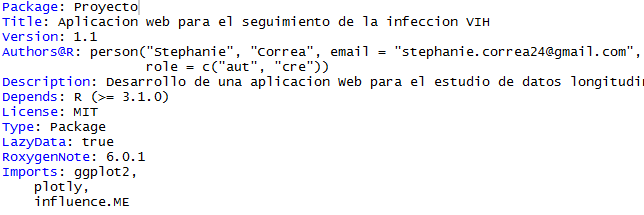
\includegraphics[scale=1]{description.PNG}
\caption{Configuraci\'on b\'asica de la aplicaci\'on }
\end{figure}

\subsubsection{Archivo NAMESPACE}

El archivo NAMESPACE lo crea RStudio, en base al archivo DESCRIPTION previamente creado, es de vital importancia este archivo, porque representa la autenticidad del paquete ante otros paquetes. Se genera al utilizar la siguiente expresi\'on:

\begin{figure}[H]
 \centering
 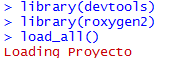
\includegraphics[scale=1]{creacion.png}
 \caption{Creaci\'on de los manuales del paquete}
 \end{figure}
  
 Se realizaron 3 archivos .R:

\begin{itemize}
\item global.R
\item ui.R
\item server.R
\end{itemize}

Por \'ultimo, se realiz\'o el reporte que debe seguir la extensi\'on .Rmd, siguendo la metodologu\'ia del paquete Knitr, paquete que ayuda a la implementaci\'on del reporte en varios formatos. \\

El archivo global.R contiene todas las librerias asociadas para que funcione la aplicaci\'on, y la carga de los archivos asociados a la carga y visualizaci\'on del mapa.\\

El archivo ui.R contiene la estructura gr\'afica que muestra la aplicaci\'on, con los m\'odulos antes expuestos, se procedi\'o a crear la estructura b\'asica, con el diseño planteado por el wireframe, basado en la experiencia de usuario; conteniendo una estructura sencilla y funcional.\\

El archivo server.R contiene todos los c\'alculos y analisis estad\'istico, relativos a la aplicaci\'on, cada m\'odulo realizado en el archivo ui.R tiene una funci\'on relacionada, con la elaboraci\'on y construcci\'on de cada m\'odulo. server.R contiene una funci\'on que recibe todas la entradas y salidas relativas del archivo ui.R. \\

Se realiz\'o el plan de desarrollo para realizar la codificaci\'on de la aplicaci\'on.   

\section{Etapa 3}

Se desarrollo la construcci\'on de los archivos antes mencionados, con la elaboraci\'on de las funciones pertinentes para elaborar los diferentes modulos.

\subsection{Manejo de versiones}
Se desarroll\'o el  \textit{software} en \textit{RStudio}, y se procedi\'o a realizar un control de versiones de la aplicaci\'on por medio de las herramientas  \textit{Git} y  \textit{GitHub}, lo que permiti\'o un mejor manejo de lo realizado en cada etapa de la investigaci\'on.

\begin{figure}[H]
\centering
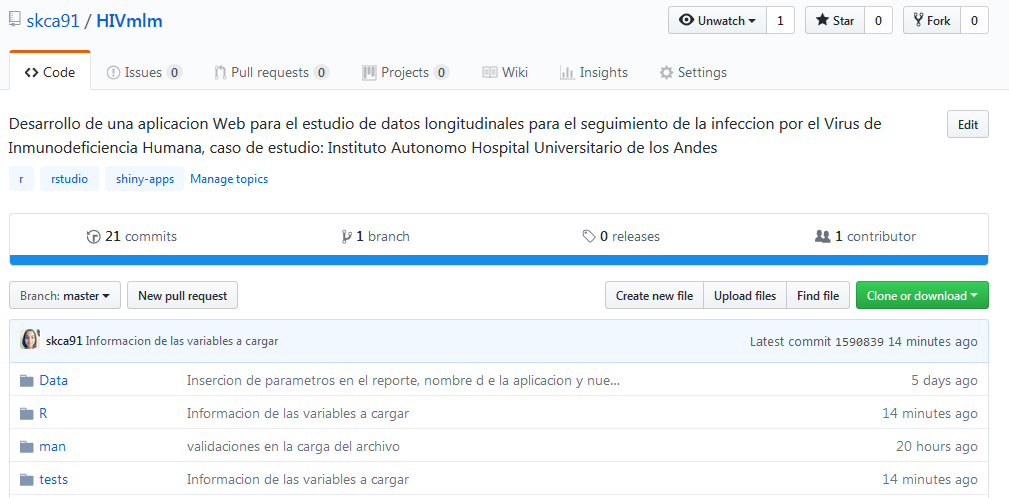
\includegraphics[scale=0.6]{github.png}
\caption{Cuenta alojada de GitHub de la aplicaci\'on}
\end{figure}


\subsection{Filtrado de los datos}

Se ha trabajado con datos recogidos por el Instituto Aut\'onomo Hospital Universitario de los Andes del estado M\'erida, desde el per\'iodo 2007-1 hasta el 2013-2. Los datos registrados, en el per\'iodo de estudio, son 1610. Los casos de VIH se han asignado a partir de la fecha de inicio del tratamiento, y en caso de no saberse, por la fecha de declaraci\'on. Se ha agregado la incidencia cada 6 meses (semestres), formando as\'i dos series temporales por año.\\

Antes del filtrado de la informaci\'on, se usaron datos de prueba para los diferentes pruebas con respecto a la carga del archivo, para esta carga se necesitaba un archivo con extension .csv, con cabecera bien definida dentro del archivo y los nombres de las variables que se necesitaban para la implementaci\'on, se conto con un archivo de extension .R, archivo usado para la creaci\'on del archivo .csv, una vez obtenido el archivo, se procedio a la carga de la informaci\'on en la aplicaci\'on.
\\

Una de las limitaciones en la carga de los archivos es la extensi\'on, solo acepta extensi\'on .csv, siguiendo unas reglas definidas, con respecto a los nombres de las variables.
\\

En esta etapa se logr\'o la elaboraci\'on del m\'odulo de la carga de datos, luego de realizar varias pruebas, en este caso, se logr\'o el prototipo 1 y los objetivos planteados para este prototipo, logrando as\'i planificar la nueva etapa.
\\

\begin{figure}[H]
\centering
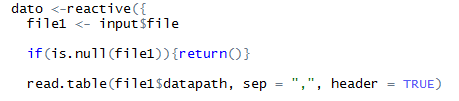
\includegraphics[scale=0.8]{archivo2.PNG}
\caption{Implementaci\'on en R de la carga de archivo}
\end{figure}

Para el desarrollo del m\'odulo de Exploraci\'on de datos, se usaron las librer\'ias de R, plotly y ggplot2.\\

\subsection{Exploraci\'on de datos}

Este m\'odulo esta compuesto por 3 secciones, que comprende el g\'enero, la edad y las cargas con respecto a la carga viral plasm\'atica, las c\'elulas $T^{+}CD4$ y c\'elulas $T^{+}CD8$; para la elaboraci\'on de la categor\'ia por g\'enero, primero se filtraron los datos por per\'iodos, tenemos los per\'iodos de 20071 hasta 20132, cada per\'iodo esta comprendido por semestres, es decir, un año esta compuesto por dos per\'iodos, en este caso, se filtr\'o la informaci\'on, para omitir los datos faltantes con respecto a la muestra de la carga viral plasm\'atica, es decir, solo se tomaron en cuenta, los pacientes que tuvieron un registro por cada per\'iodo, tomando como resultado la cantidad de hombres y mujeres que asistieron al tratamiento durante determinado per\'iodo; se logr\'o con la implementaci\'on del  algoritmo que se muestra en la figura 4.5. 

\begin{figure}[H]
\centering
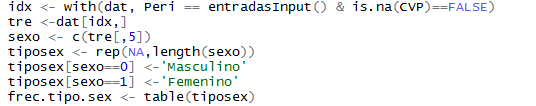
\includegraphics[scale=1]{algoritmo.png}
\caption{Algoritmo usado para filtrar la informaci\'on}
\end{figure}

Se implementaron   paneles  para dividir los diferentes gr\'aficos obtenidos.

Se implement\'o un gr\'afico de torta para sectorizar el g\'enero con respecto a los infectados con VIH. Se utilizo la siguiente funcion para su codificaci\'on.

\begin{figure}[H]
\centering
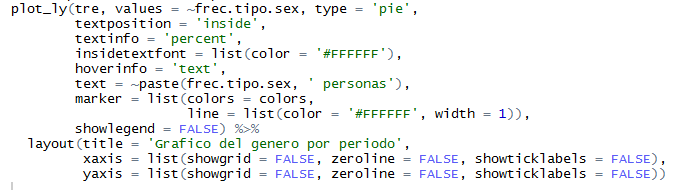
\includegraphics[scale=0.8]{torta.PNG}
\caption{Implementaci\'on en R del gr\'afico de torta}
\end{figure}

En la categor\'ia por la edad, se realiz\'o un histograma, y la debida implementacion del c\'odigo en R (Figura 4.7). Se realizo un filtro antes de realizar la graficaci\'on.

\begin{figure}[H]
\centering
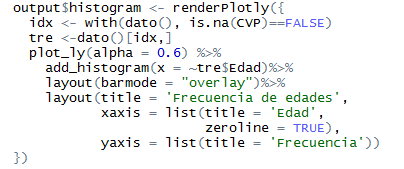
\includegraphics[scale=0.8]{histogram.PNG}
\caption{Implementaci\'on en R del histograma}
\end{figure}

En la categor\'ia por las cargas, para la mejor visualizaci\'on de los datos, se utiliz\'o un gr\'afico de puntos (Figura 4.8), las variables que son indispensables son la carga viral plasm\'atica, las c\'elulas $T^{+}CD4$ y $T^{+}CD8$. \\

\begin{figure}[H]
\centering
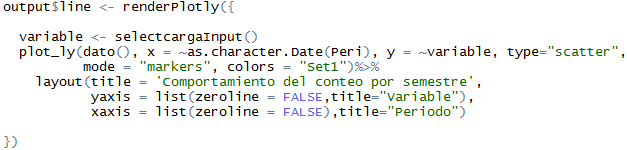
\includegraphics[scale=0.8]{ca.PNG}
\caption{Implementaci\'on en R de la selecci\'on de las cargas}
\end{figure}

Las limitaciones con respecto a la exploraci\'on de datos, son los datos faltantes, por lo cual, se aplicaron los debidos filtros para omitir dichos datos.\\

\subsection{Ajuste del modelo}

Se planific\'o la elaboraci\'on de los m\'odulos de Ajuste del m\'odelo y Validaci\'on del m\'odelo. El an\'alisis de las tendencias mostradas en los m\'odulos, se implement\'o mediante las librer\'ias de R, lm4, influence.ME, nlme y lmerTest.\\

En el m\'odulo Ajuste del m\'odelo, se realiz\'o el estudio de los datos longitudinales, las variables CVP, CD4 y CD8 son las utilizadas para aplicar el m\'odelo lineal mixto, cada paciente presenta varias m\'edidas de estas variables, con respecto a los años, las medidas  NA representan los datos faltantes, que indican que un  paciente decidio no ir mas al programa (patron mon\'otono)  o falta de forma intermitnte (patron no mon\'otono), esta es una de las razones que permite la utilizaci\'on de un modelo lineal de efectos mixtos, ya que esta t\'ecnica permite manejar, la alta heterogeneidad entre e intra pacientes, la correlaci\'on ente las medidas de un mismo paciente, as\'i como los datos faltantes.\\

Se emple\'o la formula del m\'odelo lineal mixto para hallar los valores asociados.

\begin{figure}[H]
\centering
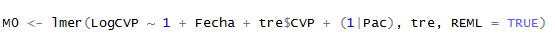
\includegraphics[scale=1]{formula.png}
\caption{F\'ormula utilizada en el m\'odelo lineal mixto}
\end{figure}

El resultado de esta formula esta ajustado por REML.\\

\subsection{Validaci\'on del modelo}

El resultado gr\'afico corresponde a los resultados obtenidos en la formula de los modelos mixtos, y corresponde a la variaci\'on de los datos cargados en la aplicaci\'on (Figura 4.10).

\begin{figure}[H]
\centering
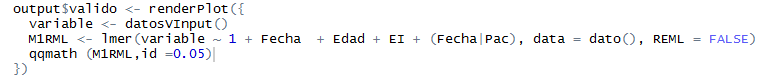
\includegraphics[scale=0.8]{validacion.PNG}
\caption{Implementaci\'on de los residuos de la validaci\'on del modelo}
\end{figure}
 
\subsection{Generaci\'on del reporte}

Se genero un archivo con extensi\'on .Rmd llamado reporte.Rmd, con la finalidad de crear el reporte en formato que se pueda guardar y el usuario pueda revisar y analizar los datos, se utilizo la siguiente estructura b\'asica para la generaci\'on del reporte (Figura 4.11).

\begin{figure}[H]
\centering
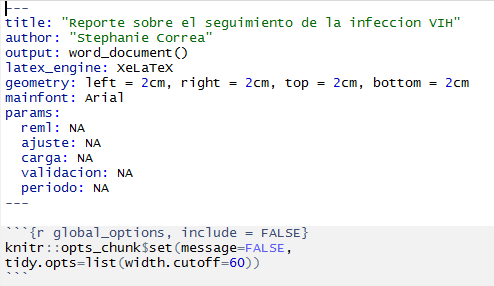
\includegraphics[scale=0.8]{reporte.PNG}
\caption{Estructura b\'asica del archivo reporte.Rmd}
\end{figure}

\subsection{Visualizaci\'on en el mapa}

Para la visualizaci\'on del mapa, se realizo la siguiente implementaci\'on de c\'odigo.

\begin{figure}[H]
\centering
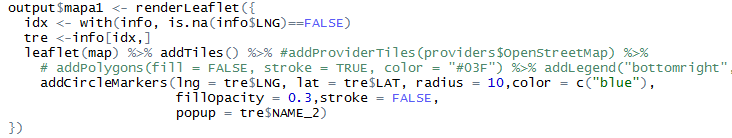
\includegraphics[scale=0.8]{mapa.PNG}
\caption{Implementaci\'on en R de la visualizaci\'on del mapa}
\end{figure}

 
En esta etapa se estableci\'o un plan de integraci\'on y pruebas, en caso de las pruebas unitarias, se realizaron en 2 fases, la primera con datos sint\'eticos que permitan comprobar cada estado del diagrama de flujo, que esquematiza la soluci\'on num\'erica que permite el c\'alculo de cada uno de los \'indices fisiol\'ogicos para entre otra herramientas pueden utilizarse los paquetes de R \emph{RUnit} \textit{\citet{runit}} y \emph{testthat} \citet{test}, y la segunda etapa donde cada funci\'on asociada a un \'indice fisiol\'ogico se le realizan prueban con los conjuntos de datos de prueba que formaran parte integral del paquete y con los cuales se desarrollaran los ejemplos pr\'acticos que conformaran la documentaci\'on que acompaña al paquete R.\\

\section{Etapa 4}
    
La etapa 4 esta compuesta  solo por 3 fases, ya que en esta etapa se ha obtenido el prototipo operativo, el cual se han implementado las diferentes pruebas de caja blanca y caja negra.\\

En la etapa anterior, se realiz\'o un plan de integraci\'on y pruebas, donde se estableci\'o la utilizaci\'on de las herramientas \textit{RUnit} y \textit{testthat}. \\

La implementaci\'on de la aplicaci\'on es la creaci\'on completa del paquete en R, donde el usuario puede descargar el paquete desde RStudio y utilizar la aplicaci\'on HIVmlm.

\begin{figure}[H]
\centering
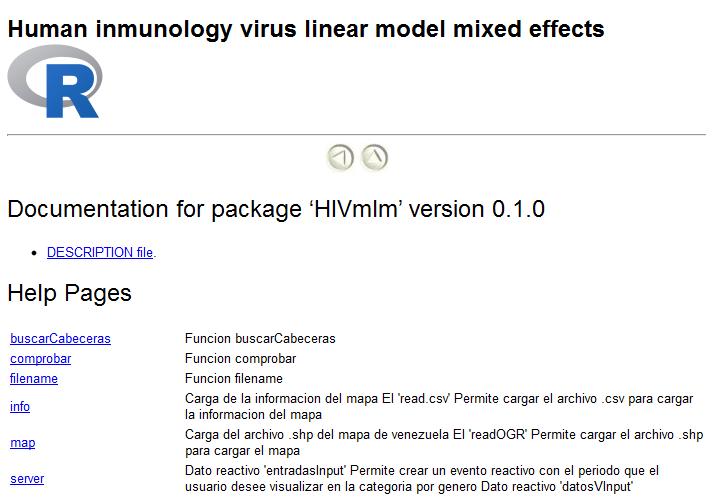
\includegraphics[scale=0.8]{HIVmlm.PNG}
\caption{Paquete cargado en las librerias de R}
\end{figure}








 
